\section{Result}

\subsection{Simulated Environment}

Figure \ref{figure/convergence} illustrates the convergence in one optimization run with the optimal hyperparameters. A mean loss of approximately -1 in an environment where the optimizer might not even be able to find the best solution seemed promising. To validate the observation, the simulation has been modified to only sample randomly. The results indicated that the previously observed low mean losses might not be that impressive. In an exemplary simulation, random sampling yielded a loss of -2.679 over 100 runs. Which is worse than sampling with the developed Bayesian optimization algorithm, but not too far off. Increasing the amount of to-optimize parameters from 3 to 5 was anticipated to yield a starker difference between the developed algorithm and random sampling. However, the results were similar to previous comparisons: The Bayesian optimization algorithm was better than random sampling but only by a small margin. To conclude the results of the simulation: The developed optimization algorithm comes consistently close to the optimal solution in a simulated environment, but the performance might not be much better than random sampling.

\begin{figure}[h]
    \centering
    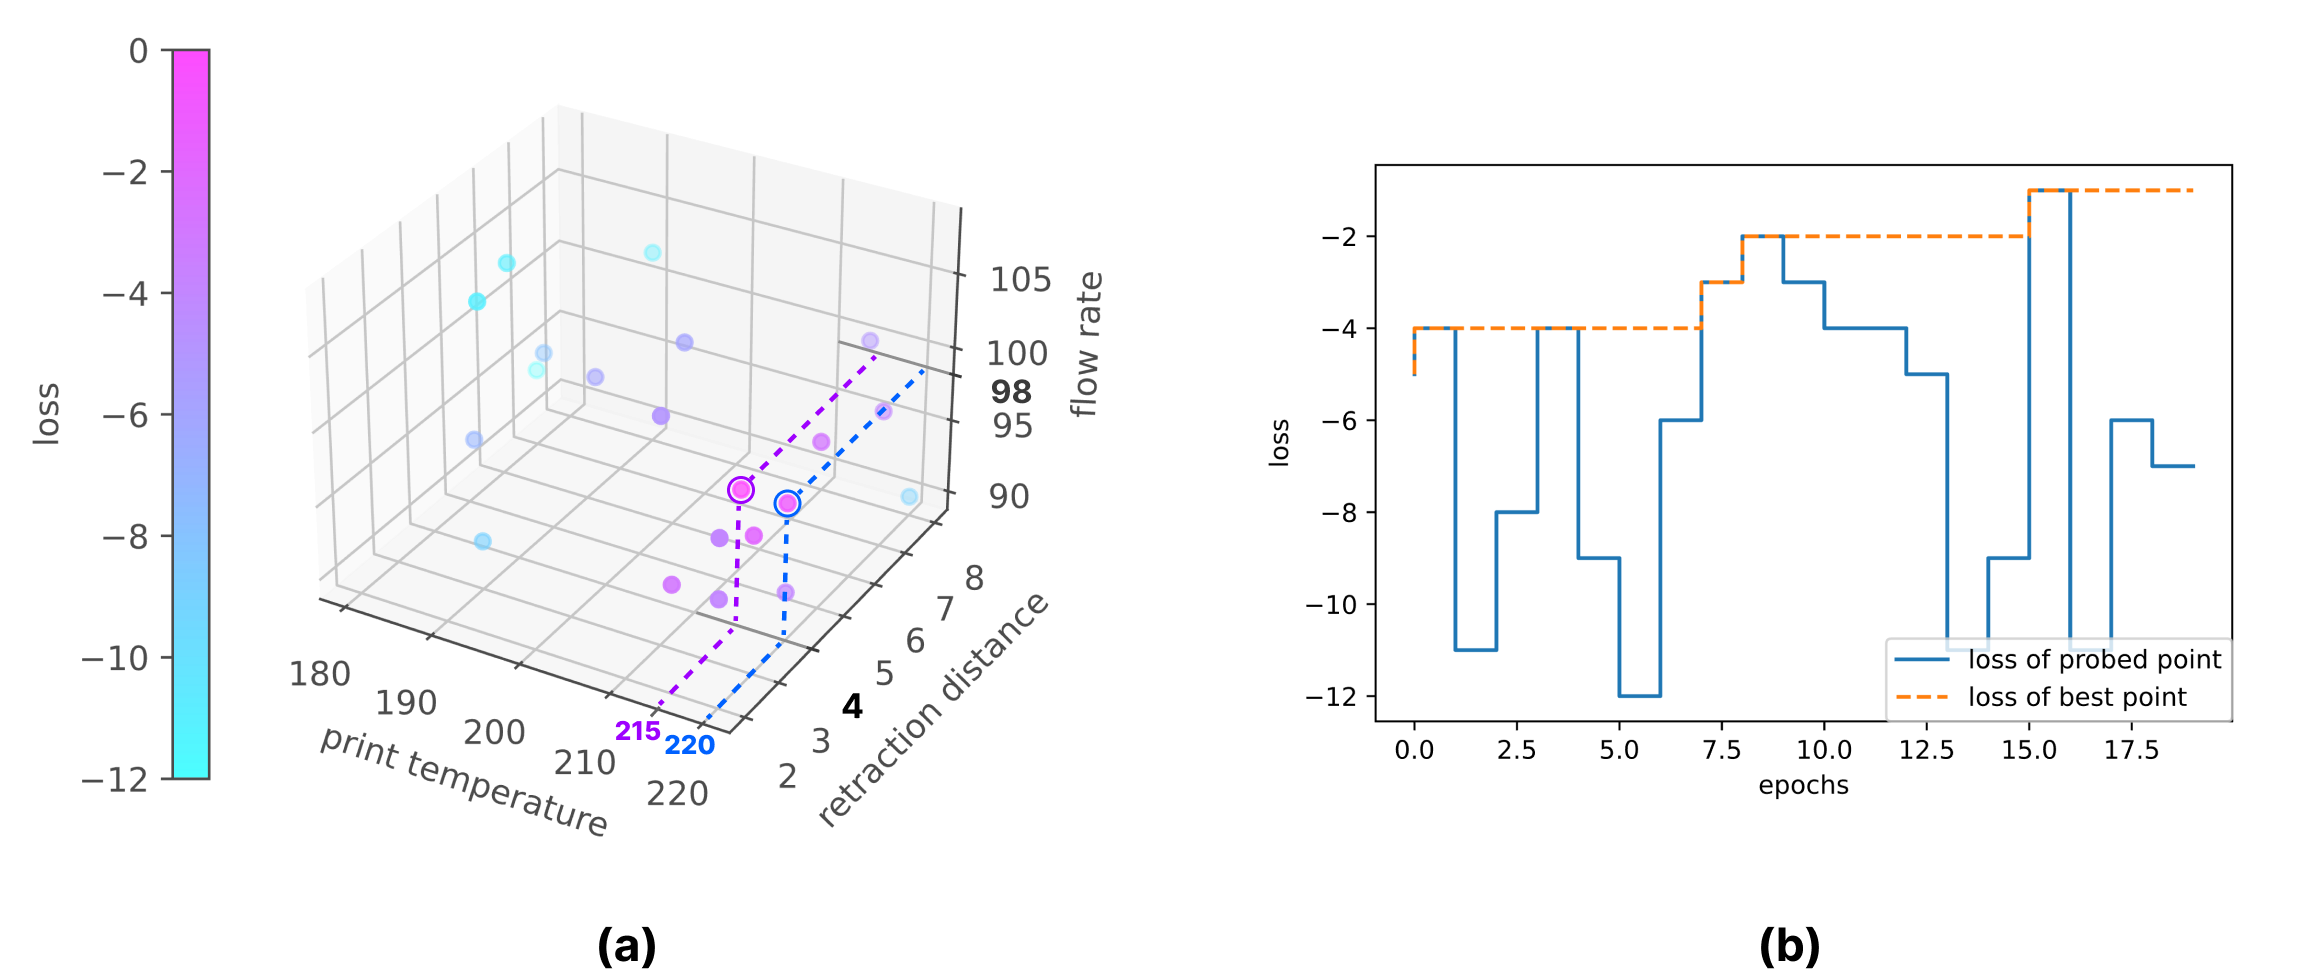
\includegraphics[width=1\linewidth]{assets/convergence_both.png}
    \caption{(A) and (b) show the convergence process of the implementation in one particular run in which the truth value has been defined as (215 print temperature, 4 retraction distance, 98 flow rate). Figure (a) shows all probes points and their loss. The dot marked with the purple outline and purple dotted lines is the truth value while the dot marked with a blue outline and blue dotted lines is the point determined to be the best after the optimization process. Figure (b) shows the loss in each epoch (of each probed point in order) and the best known point so far of the same optimization process.}
    \label{figure/convergence}
\end{figure}

\subsection{Real-World Evaluation}

The printer used for real-world evaluation was a Creality Ender 3, one of the most recommended and sold 3D printers with a price tag that's below \$250 \cite{buyersGuideEnder, buyersGuideEnder2}. The printer has been upgraded with a glass print bed and motor silencers. None of which are expected to influence the the evaluation in a meaning-full manner. PLA has been used as filament as it is the most used material for 3D printing \cite{statistaMaterial}. 
The selected test object is the "Smart compact temperature calibration tower" from Zolee Gaa \cite{smartCalibrationTower}. The object has been chosen since it tests multiple test patterns at once, namely overhangs, bridges, stringing and curvy shapes, in about 19 minutes per test print. Figure \ref{figure/smartCalibrationTowerSegment} shows the object. 

The result was two-folded: First, the fact of just printing test objects without thinking what settings could or should be changed next is convenient, so much so that even the long time it took to finish one optimization process (roughly 6 hours / 15 test prints) was not too problematic. But, the improvement was diminishing small. Too small to justify 6 hour long optimization processes. The improvement might be higher, the more variables are optimized. However, each added variable is expected to lengthen the optimization process disproportionately which has been shown in the evaluation of the simulation.  

\begin{figure}[b]
    \centering
    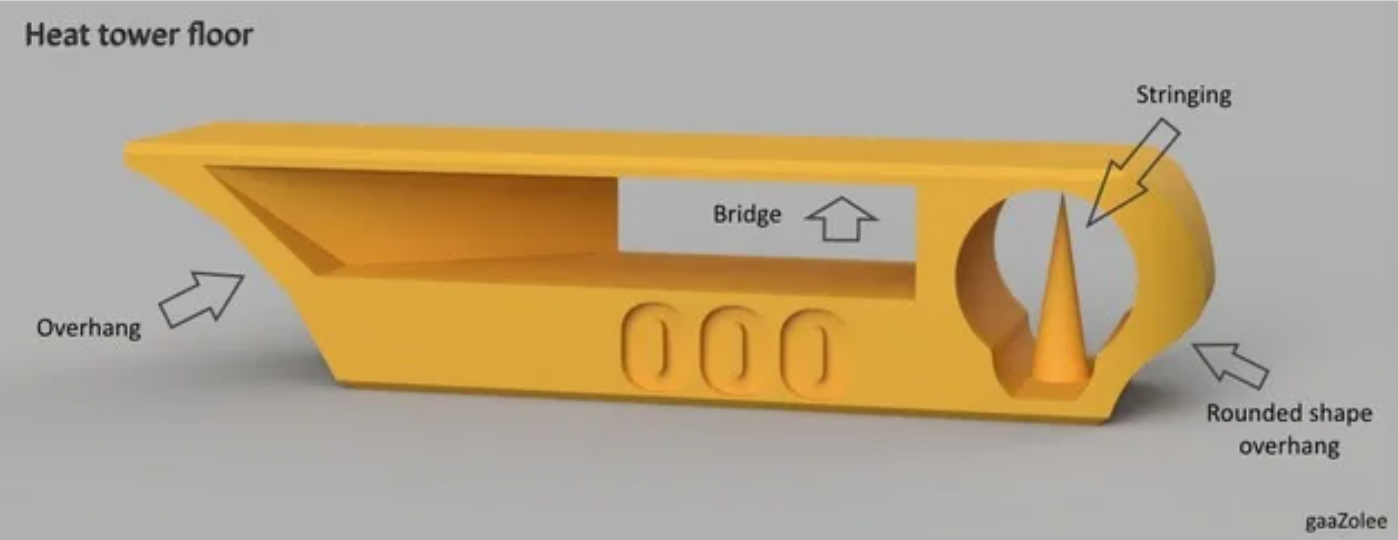
\includegraphics[width=0.65\textwidth]{assets/smartCalibrationTowerSegment.png}
    \caption{The test object used to evaluate the implementation under real circumstances. The particularity of this object is that it tests multiple common print defects in under 20 minutes. The figure has been taken from \cite{smartCalibrationTower}.}
    \label{figure/smartCalibrationTowerSegment}
\end{figure}